% samplepaper.tex: springer.com
% modificato da MM 06/05/2018
%
\documentclass[runningheads]{llncs}
\usepackage[italian]{babel}
\usepackage{graphicx}
\usepackage{subfigure}
% Used for displaying a sample figure. If possible, figure files
% should be included in EPS format.  If you use the hyperref package,
% please uncomment the following line to display URLs in blue roman
% font according to Springer's eBook style:
% \renewcommand\UrlFont{\color{blue}\rmfamily}
\begin{document}
%
\title{Organizzazione e contenuti della relazione di mini-progetto}
%
% \titlerunning{Abbreviated paper title}
% If the paper title is too long for the running head, you can set
% an abbreviated paper title here
%
\author{%
  Primo Autore\inst{1} \and
  Secondo Autore\inst{2,3} \and
  Terzo Autore\inst{3}}
%
\authorrunning{P. Autore et al.}
% First names are abbreviated in the running head.  If there are more
% than two authors, 'et al.' is used.
%
\institute{Corso di laurea in Statistica per le tecnologie e le scienze,
  matricola 1234567 \email{primo.autore@studenti.unipd.it} \and Corso
  di laurea in Statistica, economia e impresa, matricola 2345678
  \email{secondo.autore@studenti.unipd.it} \and Corso di laurea
  per le tecnologie e le scienze, matricola 3456789
  \email{terzo.autore@studenti.unipd.it}\footnote{Si veda alla fine come aggiungere le
    proprie foto.}}
%
\maketitle        
% typeset the header of the contribution
%
\begin{abstract}
  Qui si scrive il riassunto del tema, del problema specifico
  affrontato, dell'approccio seguito e dei risultati principali. Si
  mettano anche dei termini chiave qui sotto.  \keywords{{\it
      Information Retrieval} \and statistica \and ...}
\end{abstract}

\section{Introduzione}
\label{sec:introduzione}

L'obiettivo principale della relazione \`e da una parte la
documentazione del progetto di un servizio di {IR} e dall'altra una
misura del grado in cui si sia riusciti a mettere in pratica i
contenuti della disciplina illustrati durante le lezioni.  

A tal scopo la relazione dovr\`a illustrare nelle sezioni successive:
\begin{itemize}
\item i metodi di indicizzazione,
\item i modelli di reperimento,
\item l'interfaccia basata su un \textit{browser} per il {WWW}
\item i risultati della \emph{valutazione} condotta con la collezione
  sperimentale OHSUMED.
\end{itemize}
Il lettore della relazione \`e lo studente medio di un corso di laurea
in statistica al quale la relazione deve dare tutti gli strumenti per
comprendere il contenuto.  Ci si metta nei suoi panni e si scriva
tutto ci\`o e solo ci\`e che serve.  Chiedersi qual \`e il messaggio
che lo studente deve ``portarsi a casa'', esplicitarlo in questo
paragrafo e concentrarsi su quello nel resto della relazione.

L'introduzione della relazione deve servire al lettore a capire se
vale la pena continuare a leggere il resto.  Si possono riassumere i
contenuti delle sezioni successive e metterne in evidenza i punti
principali.  La relazione consiste di tre paragrafi principali dopo
questa introduzione e prima della bibliografia, per la quale si
suggerisce Bib\TeX\ se si scrive con \LaTeX.

\section{Base di partenza}
\label{sec:base-di-partenza}

La base di partenza \`e formata dai metodi documentati nei libri di
testo.  Si eviti di trascrivere pari pari, si cerchi piuttosto di
rielaborare i contenuti in modo da renderli \emph{coerenti} col resto
della relazione; in particolare, si descrivano tutti e solo i metodi
usati negli esperimenti e si eviti di parlare di quei metodi che poi
non sono stati usati; ad esempio, se si conducono degli esperimenti
con BM25F, si deve descrivere questo schema di pesatura in questa
sezione. 

\section{Metodi proposti}
\label{sec:metodi-utilizzati}

Nel caso in cui si siano sviluppati:
\begin{itemize}
\item modelli di reperimento,
\item metodi di indicizzazione,
\item schemi di pesatura o
\item altri metodi o tecniche
\end{itemize}
propri, non documentati in libri di testo o altra letteratura, si
scriva in questa sezione una descrizione accurata e completa.  Si
mettano in evidenza le caratteristiche distintive dei propri
contributi.  Se non si \`e proposto nulla di nuovo, si scriva
\emph{Nessuno}.  In una delle ultime lezioni si vedr\`a come
implementare delle proprie funzioni di reperimento e schemi di
pesatura. 

\section{Esperimenti}
\label{sec:esperimenti}

Si descriva la collezione sperimentale OHSUMED in termini di
dimensione e tipo di dati.  Si descrivano i risultati dei confronti
tra metodi di base e/o quelli proposti.  Cruciale \`e la descrizione
accurata degli esperimenti: essa deve permetterne la replicazione.

Il \textit{software}, sia quello a titolo esemplificativo dei concetti
che quello che realizza i propri metodi, va caricato su moodle nella
cartella messa a disposizione pi\`u avanti.  Nella relazione va
scritta la descrizione dell'algoritmo in modo preciso e completo da
permetterne la riproduzione.

\begin{thebibliography}{8}
\bibitem{ref_article1}
Autore, F.: Article title. Journal \textbf{2}(5), 99--110 (2016)

\bibitem{ref_lncs1}
Autore, F., Autore, S.: Title of a proceedings paper. In: Editor,
F., Editor, S. (eds.) CONFERENCE 2016, LNCS, vol. 9999, pp. 1--13.
Springer, Heidelberg (2016). \doi{10.10007/1234567890}

\bibitem{ref_book1}
Autore, F., Autore, S., Autore, T.: Book title. 2nd edn. Publisher,
Location (1999)

\bibitem{ref_proc1}
Autore, A.-B.: Contribution title. In: 9th International Proceedings
on Proceedings, pp. 1--2. Publisher, Location (2010)

\bibitem{ref_url1}
LNCS Homepage, \url{http://www.springer.com/lncs}. Last accessed 4
Oct 2017
\end{thebibliography}

\begin{figure}[h!]
  \subfigure[Primo Autore]{
    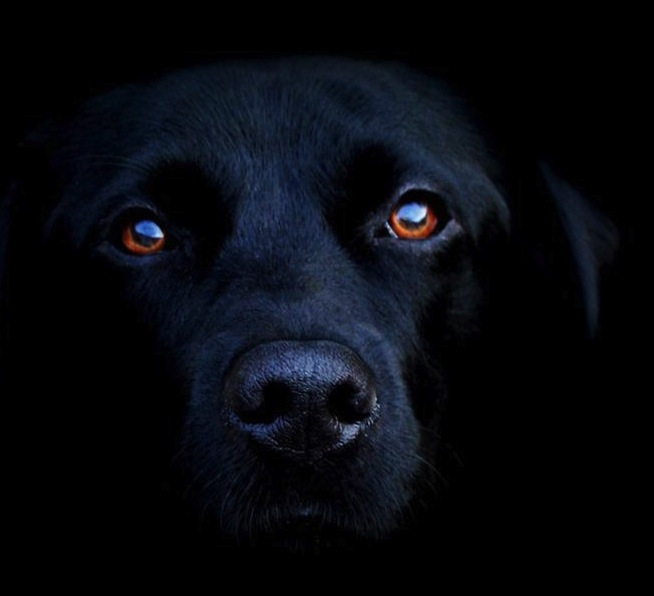
\includegraphics[width=30mm,height=30mm]{dog}}
  \subfigure[Secondo Autore]{
    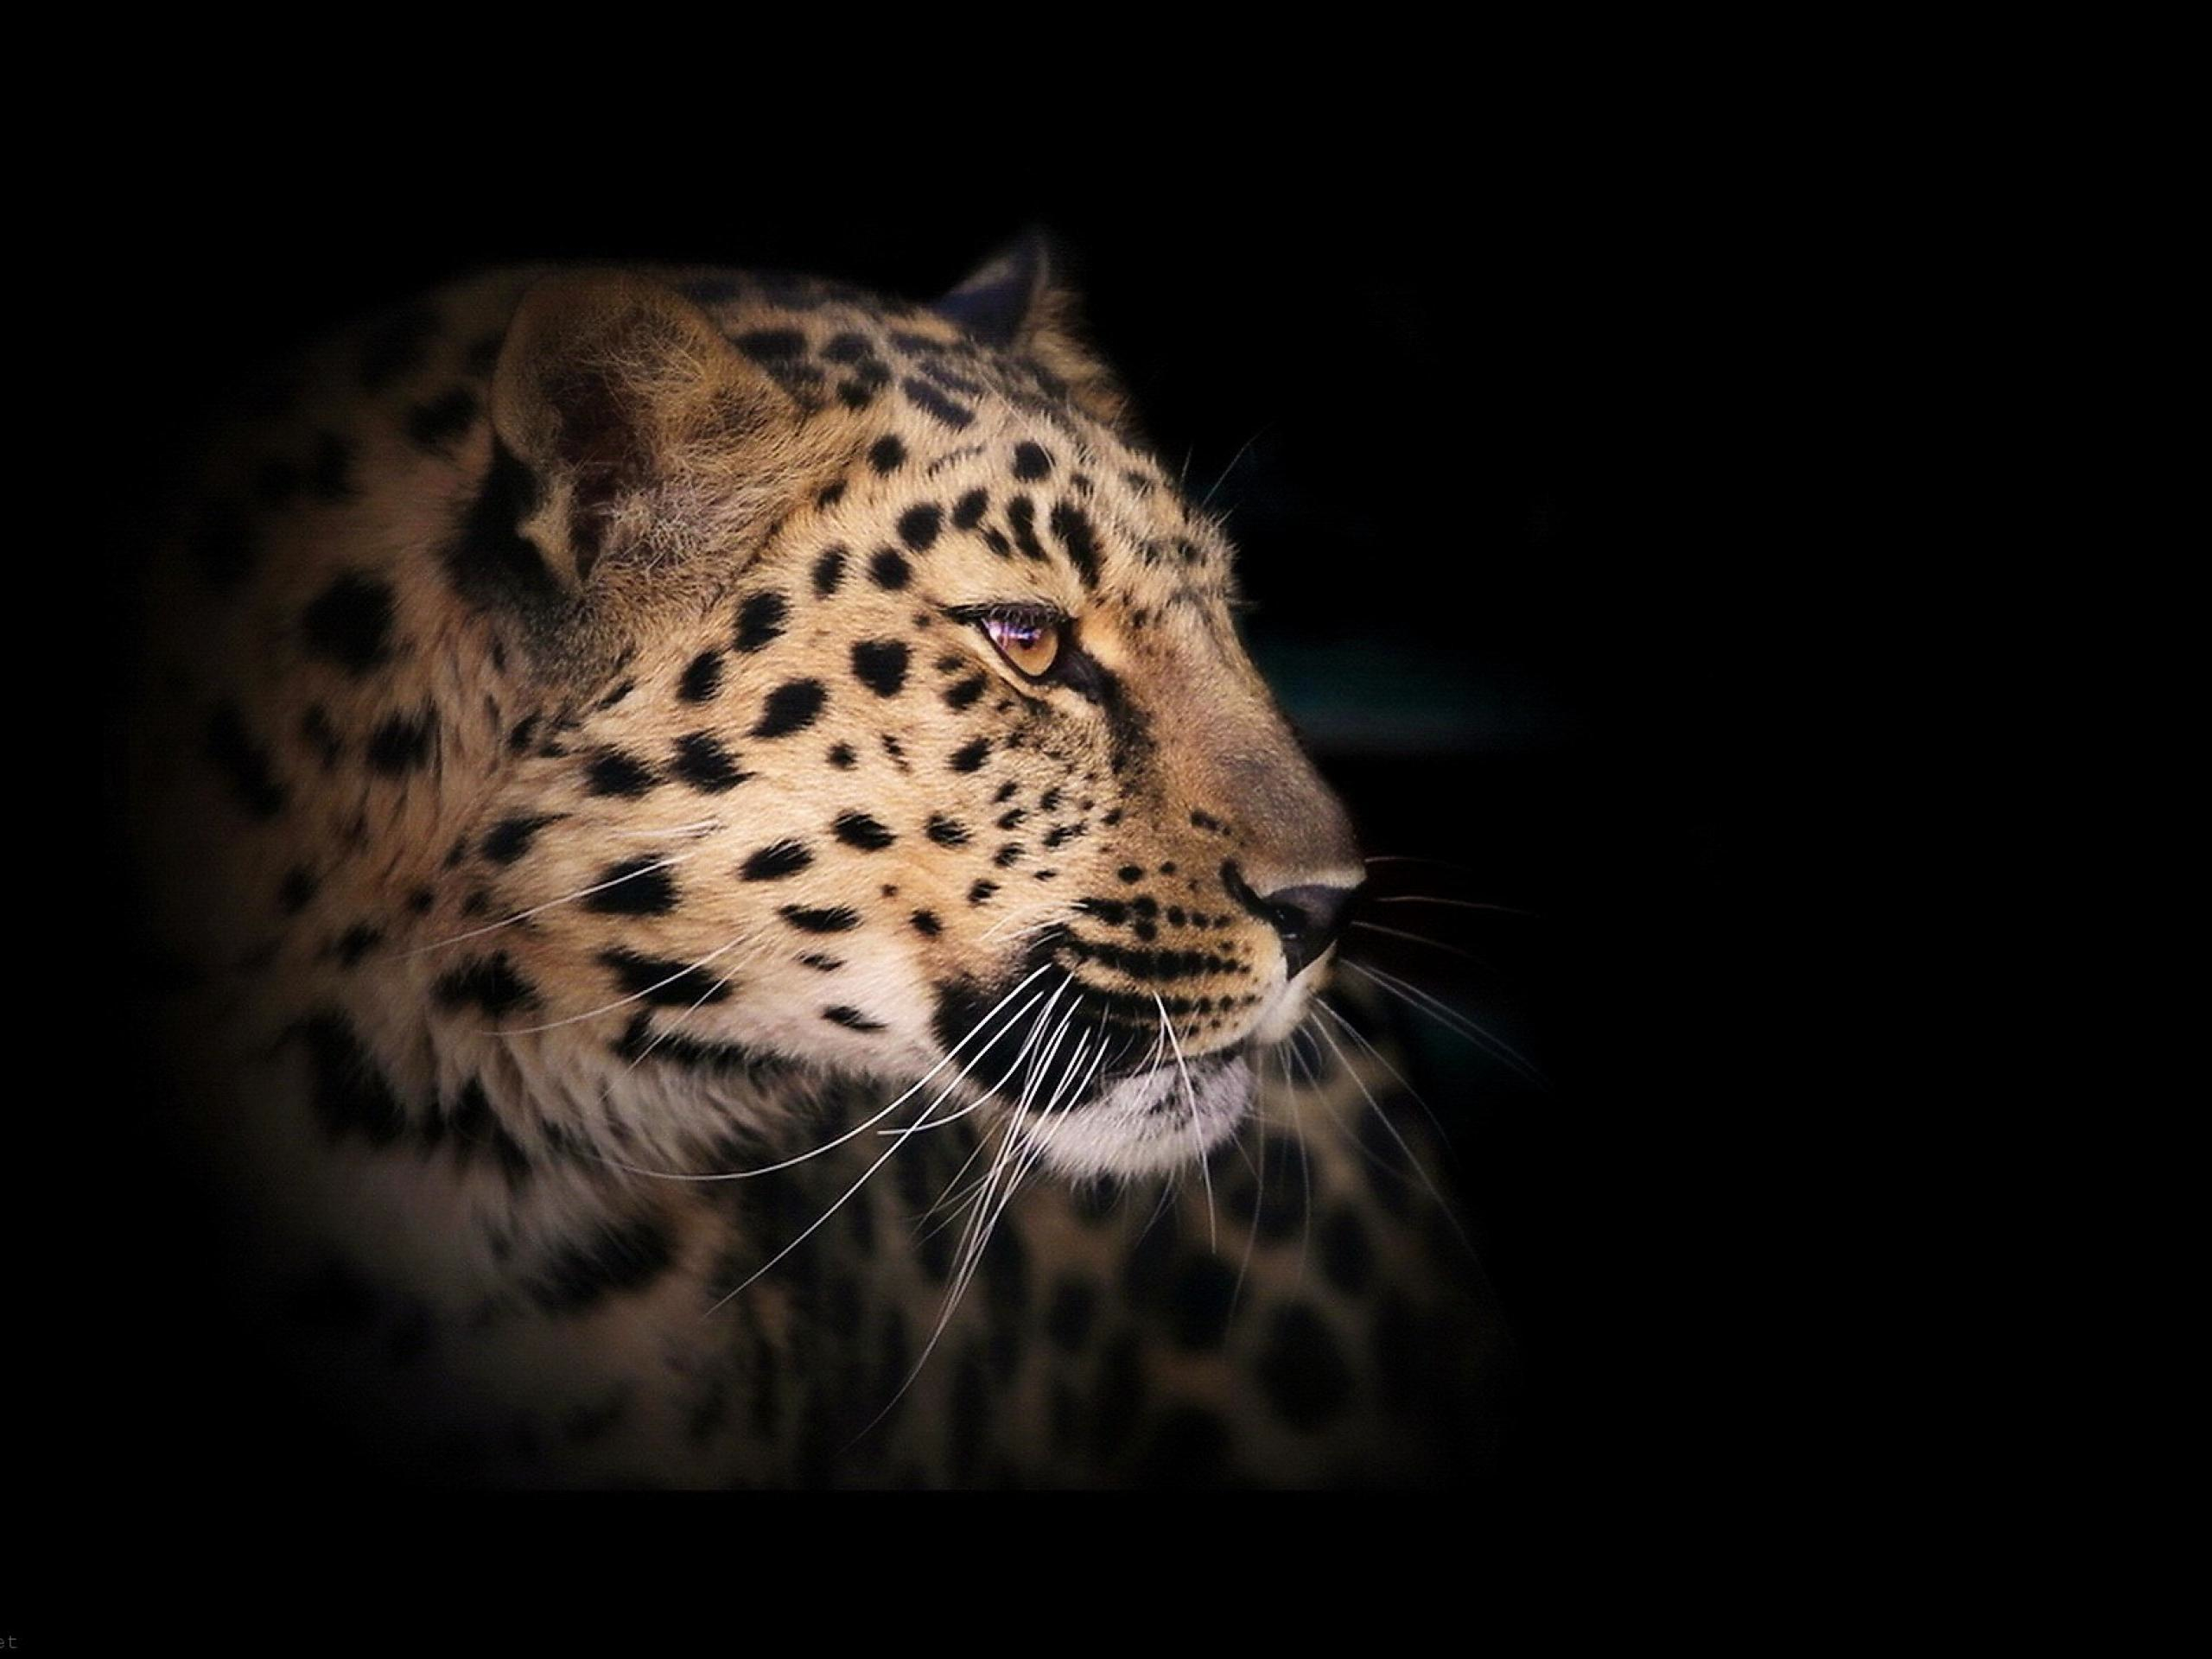
\includegraphics[width=30mm,height=30mm]{tiger}}
  \subfigure[Terzo Autore]{
    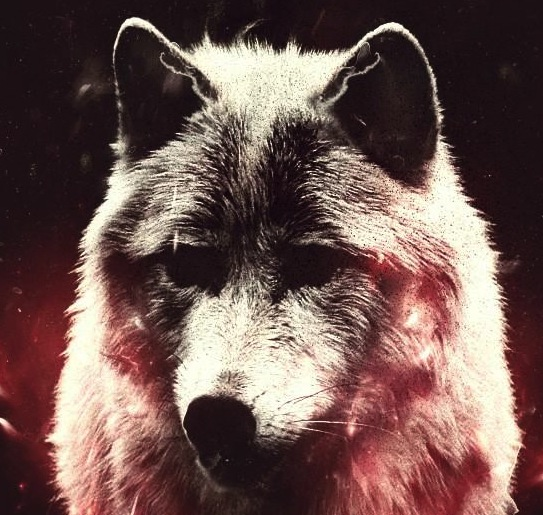
\includegraphics[width=30mm,height=30mm]{wolf}}
\end{figure}

\end{document}
